\documentclass{llncs}
% * <peter.christen@anu.edu.au> 2016-08-19T15:07:29.567Z:
%
% ^.
%\usepackage{llncsdoc}
\usepackage{epsfig}
\usepackage{graphicx}

%\usepackage{caption}
%\usepackage{subcaption}

\newtheorem{mydef}{Def.}
\newtheorem{myhyp}{Hypothesis}

\usepackage{url}
\usepackage{hyperref}

\pagestyle{empty}

% PAKDD 2018: maximum 12 pages
% Abstract max 200 words
% title, abstract: 1/2 page
% introduction: 1 1/2 page (2 pages so far)
% related work: 1 to 1 1/2 pages (3 pages so far)
% method: 4 pages (7 pages so far)
% experiments: 3 (10 pages so far)
% discussion /conclusion: 1 page
% citations 1

% ====================================================================

% Eamonn ICDM'10 tutorial slides
% - clear problem statement in abstract
% - To convince a reviewer, you must think like a reviewer

% Writing the paper:
% - Make a working title
% - Introduce the topic and define (informally at this stage)
%   terminology
% - Motivation: Emphasize why is the topic important
% - Relate to current knowledge: what’s been done
% - Indicate the gap: what need’s to be done?
% - Formally pose research questions
% - Explain any necessary background material.
% - Introduce formal definitions.
% - Introduce your novel algorithm/representation/data structure etc.
% - Describe experimental set-up, explain what the experiments will
%   show
% - Describe the datasets
% - Summarize results with figures/tables
% - Discuss results
% - Explain conflicting results, unexpected findings and discrepancies
%   with other research
% - State limitations of the study
% - State importance of findings
% - Announce directions for further research
% - Acknowledgements
% - References
%
% - Don’t make the reviewer of your paper think!
% - Reviewers make an initial impression on the first page and don’t
%   change 80% of the time
% - A good introduction with a good motivation is half your success
% - By the end of the introduction the reviewer mustknow.
%   - What is the problem?
%   - Why is it interesting and important?
%   - Why is it hard?why do naive approaches fail?
%   - Why hasn't it been solved before?(Or, what's wrong with previous
%     proposed solutions?)
%   - What are the key components of my approach and results?Also
%     include any specific limitations.
%   - A final paragraph or subsection: “Summary of Contributions”.
%     It should list the major contributions in bullet form,
%     mentioning in which sections they can be found. This material
%     doubles as an outline of the rest of the paper, saving space and
%     eliminating redundancy
% - Unjustified Choices (are bad)
% - Optimal: Does not mean `very good'
% - Proved: Does not mean `demonstrated'
% - Significant: There is a danger of confusing the informal statement
%   and the statistical claim
% - Use all the Space Available
% - Avoid Weak Language: aim, attempt, might, etc.
% - Use the Active Voice
% - ALWAYS put some variance estimate on performance measures (do
%   everything 10 times and give me the variance of whatever you are
%   reporting)

% Figures:
% - Don't cover the data with the labels!
% - Color helps -Direct labeling helps -Meaningful captions help
%
% Common problem with figures:
% 1.Too many patterns on bars
% 2.Use of both different symbols and different lines
% 3.Too many shades of gray on bars
% 4.Lines too thin (or thick)
% 5.Use of three-dimensional bars for only two variables
% 6.Lettering too small and font difficult to read
% 7.Symbols too small or difficult to distinguish
% 8.Redundant title printed on graph
% 9.Use of gray symbols or lines
% 10.Key outside the graph
% 11.Unnecessary numbers in the axis
% 12.Multiple colors map to the same shade of gray
% 13.Unnecessary shading in background
% 14.Using bitmap graphics (instead of vector graphics)
% 15.General carelessness

% ====================================================================

% TODO:
% - clearly point out novelty of this work
% - contribution compared to earlier work

\begin{document}

\title{Efficient and accurate record linkage using similarity spaces}
%  \thanks{The authors would like to thank the Isaac Newton Institute
%  for Mathematical Sciences, Cambridge, for support and hospitality
%  during the programme \emph{Data Linkage and Anonymisation} where
%  this work was conducted (EPSRC grant EP/K032208/1). Peter Christen
%  was also supported by a grant from the Simons Foundation. The work
%  was also partially funded by the Australian Research Council
%  (DP130101801).}}

\author{Submitted for double-blind review}
%\author{Peter Christen\inst{1} \and Rainer Schnell\inst{2}
%        \and Dinusha Vatsalan\inst{1} \and Thilina
%        Ranbaduge\inst{1}}
%\institute{Research School of Computer Science,
%           The Australian National University, \\
%           Canberra, Australia.~
%           Contact: \email{peter.christen@anu.edu.au}
%           \and
%           Methodology Research Group, %Institute for Sociology,
%           University Duisburg-Essen, Duisburg, Germany.} %~
%%           \email{rainer.schnell@uni-due.de}}

\maketitle

\begin{abstract}
% usually about 200 words max- best to check

\end{abstract}

\keywords Entity resolution; deduplication; metric spaces; etc.

% ====================================================================

\section{The Plan}

We tried to develop a plan with PeterC. Here is the photo of the white-board.

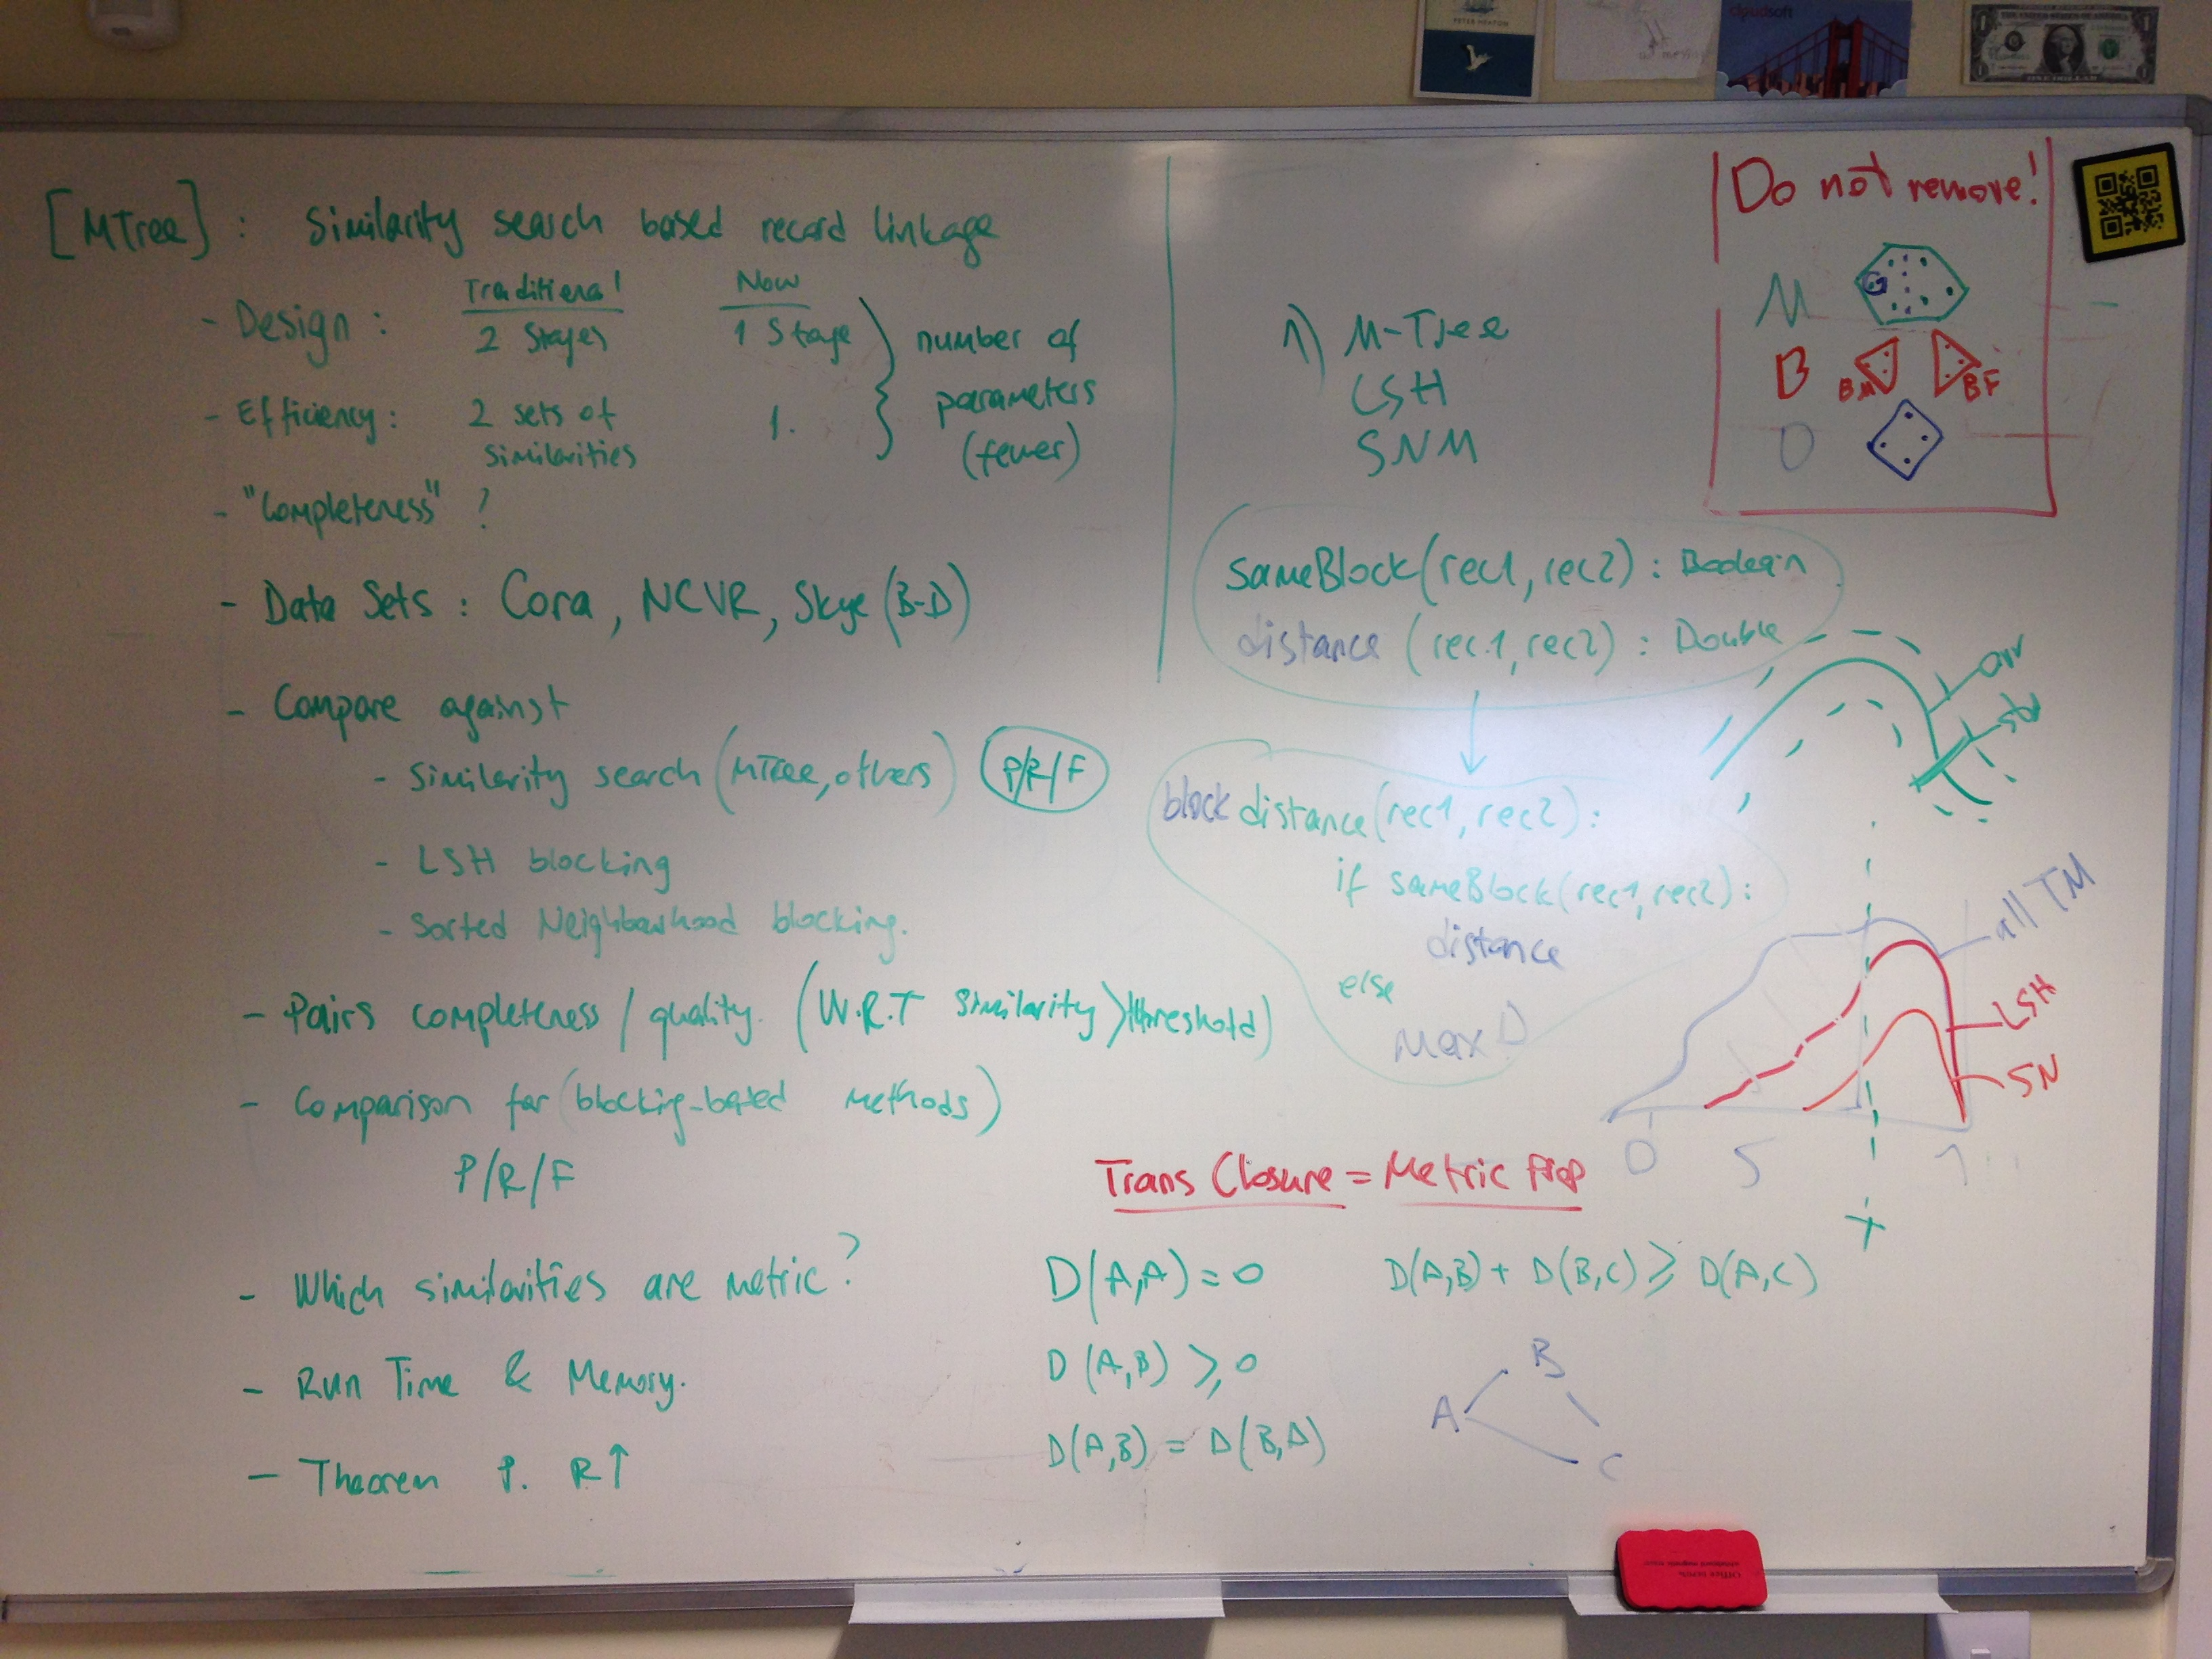
\includegraphics[width=\textwidth]{2017-08-01_12_08_43.jpg}

\vspace{5mm}

But, even better, here it is in a bulleted list.

\begin{itemize}
\item Design: Traditionally it has two stages. A blocking method needs to be developed separately from a similarity method. With similarity search based record linkage, there is only one method, and that is the similarity method.
\item Efficiency: I am not convinced of this, but Peter thinks there may be efficiency benefits. The reasoning behind this is that with blocking-based methods we would have to calculate some sort of a similarity value first. This value will only be used for blocking, and later a similarity value between candidate pairs will need to be calculated again.
\item Completeness: Similarity search based methods will be complete (with respect to the given similarity method) whereas blocking based methods (including LSH) are likely to be incomplete (there will be high-similarity pairs which are not places in the same block)
\item Data sets
\begin{itemize}
\item Kilmarnock Birth-Death
\item Skye Birth-Death
\item CORA
\item North Carolina Voter Registration DB
\end{itemize}
\item The following is a list of all methods we thought we would have to compare.
\begin{itemize}
\item Similarity search (M-Tree, others?)
\item LSH-blocking
\item Traditional blocking (e.g. Region, Surname)
\item Sorted Neighbourhood blocking
\end{itemize}
\item Pairs-completeness and pairs-quality (w.r.t high similarity instead of true-link status). I will expand on this a bit more later.
\item Comparison (for blocking based methods)
		Precision/Recall/F1-Measure
\item Which similarity methods are metric?
\item Run time and memory usage comparisons
\item Theorem. Precision might get better or worse with similarity search based methods, but recall should never get worse.
\end{itemize}

Note: The rest of this paper should be regarded as a placeholder for now.

\section{Introduction}
\label{sec-intro}

something about record linkage and its importance, application examples

drawback of existing approaches: blocking and comparisons/classification
done separately, sometimes if bad linkage quality means to go back to redo
blocking.

something about similarity spaces / metric spaces, M-trees and its
more recent advanced/improved versions, and how they have been used in
similarity search.

How our work is different from these other metric space works, and
description of our contributions

% --------------------------------------------------------------------

\section{Related Work}
\label{sec-related}

summarise related work in blocking/indexing

summarise related work in metric spaces as used in record linkage

other related works as relevant

% --------------------------------------------------------------------

\begin{figure}[t]
  \centering
%  \includegraphics[width=1.0\textwidth]{xyz.eps}
  \caption{Descriptive caption
           %as outlined in Sect.~\ref{sec-overview} and detailed in
           %Sect.~\ref{sec-bf-attack}.
           \label{fig:xyz}}
\end{figure}

\section{approach section?}
\label{sec-overview}

coverage: proportion of all rec pairs with a certain similarity
(independent of their match status) that are being generated by
a blocking  technique

transitive closure is a problem if we have a blocking technique with overlapping blocks.

define blocking: only aimed at improving computational aspects by reducing the number of record pairs to be compared


% - - - - - - - - - - - - - - - - - - - - - - - - - - - - - - - - - -

% subsection

%  - - - - - - - - - - - - - - - - - - - - - - - - - - - - - - - - - -

%\subsection

% --------------------------------------------------------------------

\begin{figure}[t]
  \begin{center}
  \begin{scriptsize}
%    \begin{footnotesize}
  \begin{tabular}{ll} \hline
\multicolumn{2}{l}{\textbf{Algorithm 1: \emph{Candidate q-gram set
  generation}} -- Steps (1a) and (1b) } \\ \hline
\multicolumn{2}{l}{Input:} \\
\multicolumn{2}{l}{- $\mathbf{V}$: Set of attribute values and their
  frequencies from a public database} \\
\multicolumn{2}{l}{- $\mathbf{B}$: Set of BFs and their
  frequencies from the sensitive database} \\
\multicolumn{2}{l}{- $l$:~\, Length of Bloom filters} \\
\multicolumn{2}{l}{- $q$:~ Length of sub-strings to extract from
  attribute values} \\  
\multicolumn{2}{l}{- $m$: Minimum frequency for BFs and attribute
  values} \\
\noalign{\smallskip}
\multicolumn{2}{l}{Output:} \\
\multicolumn{2}{l}{- $\mathbf{C}$: List of possible q-grams for each
  BF position} \\
\noalign{\smallskip}
  1:  & $\mathbf{c}^+[p] = \{\}$, $\mathbf{c}^-[p] = \{\}$,
        $1 \le p \le l$ ~~~ // Initialize list of candidate q-gram
        sets \\
  2:  & $\mathbf{V}_F = \{v \in \mathbf{V}: v.f \ge m \}$
        ~~~~~~~~~~~~~~ // Attribute values with frequency of at
        least $m$ \\
  3:  & $\mathbf{B}_F = \{\mathbf{b} \in \mathbf{B}:
        \mathbf{b}.f \ge m \}$
        ~~~~~~~~~~~~~~\,// BFs with frequency of at least $m$ \\
  4:  & $revSort(\mathbf{B}_F)$, $revSort(\mathbf{V}_F)$ ~~~~~~~~~~ 
        // Sort according to frequencies, highest first \\
  5:  & $\mathbf{A} = [(\mathbf{b}_i, v_i) : 
        \mathbf{b}_i \in \mathbf{B}_F, v_i \in \mathbf{V}_F:
        \mathbf{b}_i.f > \mathbf{b}_j.f \land v_i.f > v_j.f:
        1 \le i < j \le min(|\mathbf{V}_F |, |\mathbf{B}_F|)]$ \\
  ~  &   ~~~~~~~~~~~~~~~~~~~~~~~~~~~~~~ // Align $\mathbf{V}_F$
        and $\mathbf{B}_F$ as long as their frequencies are
        unique \\  
  6:  & \textbf{for} $(\mathbf{b}_i, v_i) \in \mathbf{A}$
        \textbf{do}: ~~~~~~~~~~~~~~~~~~~~ //  Step (1a): Get
        candidate sets of q-grams \\
  7:  & ~~~ $\mathbf{q}_i = genQGramSet(v_i, q)$ ~~~~~~~~\,//
        Convert attribute value into its q-gram set \\
  8:  & ~~~  \textbf{for} $1 \le p \le l$ \textbf{do}: 
        ~~~~~~~~~~~~~~~~~~~\, // Loop over all BF positions \\
  9:  & ~~~ ~~~ \textbf{if} $\mathbf{b}_i[p] == 1$ \textbf{then}:
        ~~~~~~~~~~~~\, // Bit at position p is 1 \\
  10: & ~~~ ~~~ ~~~ $\mathbf{c}^+[p] = \mathbf{c}^+[p] \cup
        \mathbf{q}_i$ ~~~~~~~~~~~\,// Add to set of possible
        q-grams \\
  11: & ~~~ ~~~ \textbf{else}: ~~~~~~~~~~~~~~~~~~~~~~~~~~~~~~~~ //
        Bit at position $p$ is $0$ \\
  12: & ~~~ ~~~ ~~~ $\mathbf{c}^-[p] = \mathbf{c}^-[p] \cup
        \mathbf{q}_i$  ~~~~~~~~~~~// Add to set of \emph{not}
        possible q-grams \\
  13: & $\mathbf{C} = [\,]$ ~~~~~~~~~~~~~~~~~~~~~~~~~~~~~~~~~~~~~\,
        // Step (1b): Initialize empty list of q-gram sets \\
  14: & \textbf{for} $1 \le p \le l$ \textbf{do}: 
        ~~~~~~~~~~~~~~~~~~~~~~~~\,// Loop over all BF positions to
        combine q-gram sets \\
  15: & ~~~ $\mathbf{C}.append(\mathbf{c}^+[p] \setminus
        \mathbf{c}^-[p])$ ~~~~~~~~~~~\,// Remove not possible from
        possible q-grams \\
%  15: & ~~~ $\mathbf{c}[p] = \mathbf{c}^+[p] \setminus
%        \mathbf{c}^-[p]$ ~~~~~~~~~~~~~~~~~ // Remove not possible
%        from possible q-grams \\
%  16: & ~~~ $\mathbf{C}.append(\mathbf{c}[p])$
%        ~~~~~~~~~~~~~~~~~~~~~~ // Add to list of candidates for all
%        BF positions\\
16: & \textbf{return} $\mathbf{C}$ \\
  \hline
  \end{tabular}
%  \end{footnotesize}
 \end{scriptsize}
  \end{center}
  \label{algo:step1}
\end{figure}

%  - - - - - - - - - - - - - - - - - - - - - - - - - - - - - - - - - -

\subsection{Analysis and Limitations}
\label{sec-analysis}

maybe a complexity analysis? maybe an analysis of expected 
linkage quality?

% --------------------------------------------------------------------

\section{Experiments and Results}
\label{sec-data}

plot coverage as defined above for different data sets and the different blocking techniques

x-axis: similarity threshold from 0 to 1, y-axis is coverage as a
percentage (percentage of how many record pairs with a certain similarity value are generated by a blocking technique compared to all record pairs with that similarity - how to do this? we can't do full pair-wise comparison? can we get all pairs from m-tree for a certain distance, then run them through blocking?

For M-tree etc coverage will always be 1.0, while for other blocking techniques the coverage will be < 1.0 especially as similarities
become lower.

Plots should include average coverages for a certain similarity threshold over various parameter settings - e.g. for LHS or sorted neighbourhood, as well as min/max similarities (or std-dev bands in a transparent colour), as in the below example:

%http://www.randalolson.com/2014/06/28/how-to-make-beautiful-data-visualizations-in-python-with-matplotlib/


%% old text below  ***************************************

We conducted our experimental study using real data sets from two
domains.
%
The first are a pair of North Carolina Voter Registration (NCVR) data
sets (\url{ftp://alt.ncsbe.gov/data/})
%~\footnote{Available from \url{ftp://alt.ncsbe.gov/data/}}
collected in June 2014 (the database to be attacked) and October 2016
(the public database).
%, that have increasingly large differences in their time collection
%to see how this influences re-identification accuracy.
These data sets contain over five million records of voters including
their first names, surnames, and addresses. We present results of our
attack individually on the first name
%, last name, and address attributes, 
attribute, as well as on the concatenation of the first name and
surname attributes.

\begin{figure}[!t]
  \centering
%  \includegraphics[width=0.31\textwidth]
%  {reident-bf_len-ncvoter_20140619_1}
  ~~
%  \includegraphics[width=0.31\textwidth]
%  {reident-hash_type-ncvoter_20140619_1}
  ~~
%  \includegraphics[width=0.31\textwidth]
%  {reident-q-ncvoter_20140619_1}
  \\ ~ \\
%\includegraphics[width=0.31\textwidth]
%  {reident-bf_len-ncvoter_20140619_1-3}
  ~~
%  \includegraphics[width=0.31\textwidth]
%  {reident-hash_type-ncvoter_20140619_1-3}
  ~~
%  \includegraphics[width=0.31\textwidth]
%  {reident-q-ncvoter_20140619_1-3}
\caption{Results for the NCVR data sets with first name (top)
    and combination of first and surname (bottom) for different BF
    lengths (left), different hashing methods (middle), and different
    values of $q$ (right). No BF hardening was applied.
   \label{fig:ncvr}}
\end{figure}


The parameter settings we use in our experiments are $q = [2,3,4]$
(length of sub-strings used in BF encoding), BF length
$l = [250, 500, 1000,$ $2000]$, and either the double or random
hashing method~\cite{Sch16} as described in
Sect.~\ref{sec-overview}. We calculate the number of hash functions
$k$ based on $l$ and $q$ such that the false positive rate is
minimized~\cite{Vat14c}. We also apply the BF hardening techniques
balancing and XOR-folding~\cite{Sch16}.
% as described in Sect.~\ref{sec-overview}.
We use different numbers for the most frequent attribute values
(ranked by their frequencies) to be re-identified: $|\mathbf{G}| =
[10,20,50,100]$.
%most frequent values from the public data set to be guessed.


\textbf{Discussion:}~
In Fig.~\ref{fig:ncvr} we show the results for the NCVR data sets.
% for one individual attribute (first name) in the top row, and
%three individual attributes (first name, last name, and address in
%the first three rows, respectively), and
%combined attributes of first and surnames in the bottom row.
% BFs are hardened using the balanced method.
%
As can be seen, when the BF length $l$ increases (left column) the
percentage of correct re-identifications mostly increases, as with
larger $l$ the number of q-grams mapped to a certain bit position
decreases. All values can be correctly re-identified for individual
attributes
%nearly $90\%$ of values can be correctly re-identified
%%as 1-to-1 or 1-to-many matches
when the number of frequent values is 10.
%or 20. 
Around half of all
values can still be re-identified even when values from two
attributes


\begin{table}[!t]
 %\addtolength{\tabcolsep}{-3pt}
  \caption{Comparison of re-identification results with existing BF
     attack methods.}
     \label{table:exist_approaches}
  \centering
  \begin{scriptsize}
    \begin{tabular}{llccc}
    \hline\noalign{\smallskip}
   Publication & Data set & Num BFs~ & ~1-1 corr~ & Run time
     \\ \noalign{\smallskip}\hline\noalign{\smallskip}
  Kuzu et al. (2011)~\cite{Kuz11} & NCVR first names & 3,500 & 400 &
    1,000 sec \\
  Kuzu et al. (2013)~\cite{Kuz13} & Patient names & 20 & 4 & 
    few sec \\
  ~~~~ " & ~~~~ " & 42 & 0 & $>$ week \\
  Niedermeyer et al. (2014)~\cite{Nie14}~ & German surnames & 7,580 &
    934 & $>$ days  \\
  Kroll and Steinmetzer (2015)~\cite{Kro15}~ & German names and
    locations & 100K & 44K & $>$ days \\
  Our approach & NCVR first names & 10--100 & 7--10 & 0.73--0.75 sec
    \\
  ~~~~ " & NCVR first and surnames & 10--100 & 3--6 & 1.5--1.9
  sec  \\
%  ~~~~ " & UKCD surname and address~ & 10 & 10 & 0.05 sec \\
  \noalign{\smallskip} \hline
  \end{tabular}
  \end{scriptsize}
\end{table}

% --------------------------------------------------------------------

\section{Conclusions and Future Work}
\label{sec-concl}

% --------------------------------------------------------------------

%\bibliographystyle{abbrv}
\bibliographystyle{splncs03}
\bibliography{paper} 

\end{document}

% ====================================================================
